\begin{figure*}[!htb]
	\centering
		%\hline
		\begin{subfigure}[t]{0.32\textwidth}
			\centering
			\caption{}
			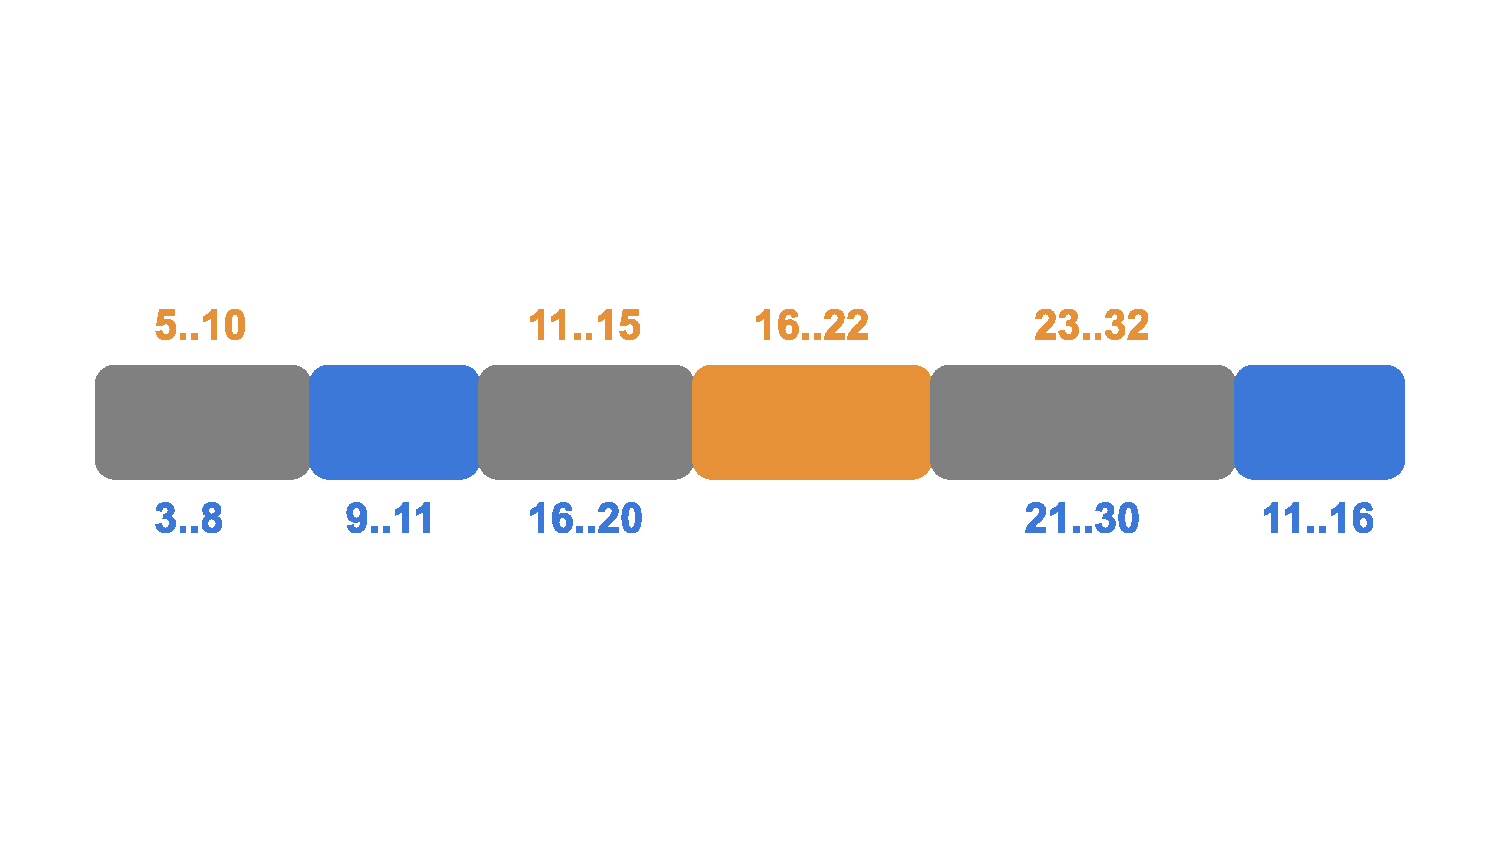
\includegraphics[width=\linewidth]{fig/sketches/1D_sketch_before_update.pdf}
			\label{fig:1d_before_update}
		\end{subfigure}
		\begin{subfigure}[t]{0.32\textwidth}
		\centering
		\caption{}
		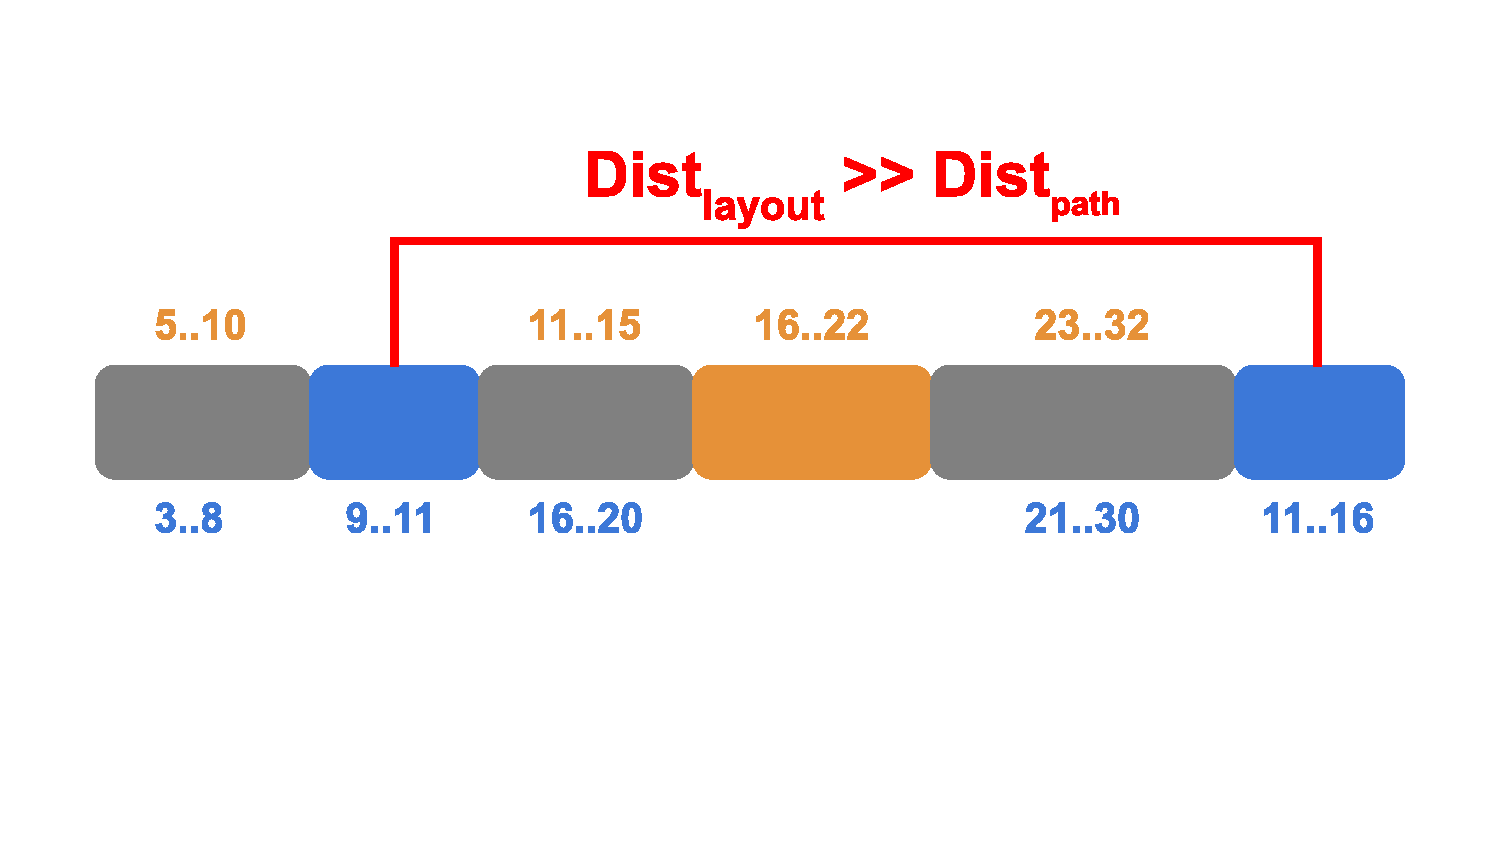
\includegraphics[width=\linewidth]{fig/sketches/1D_sketch_before_update_highlighted.pdf}
		\label{fig:1d_before_update_highlighted}
		\end{subfigure}
		\begin{subfigure}[t]{0.32\textwidth}
		\centering
		\caption{}
		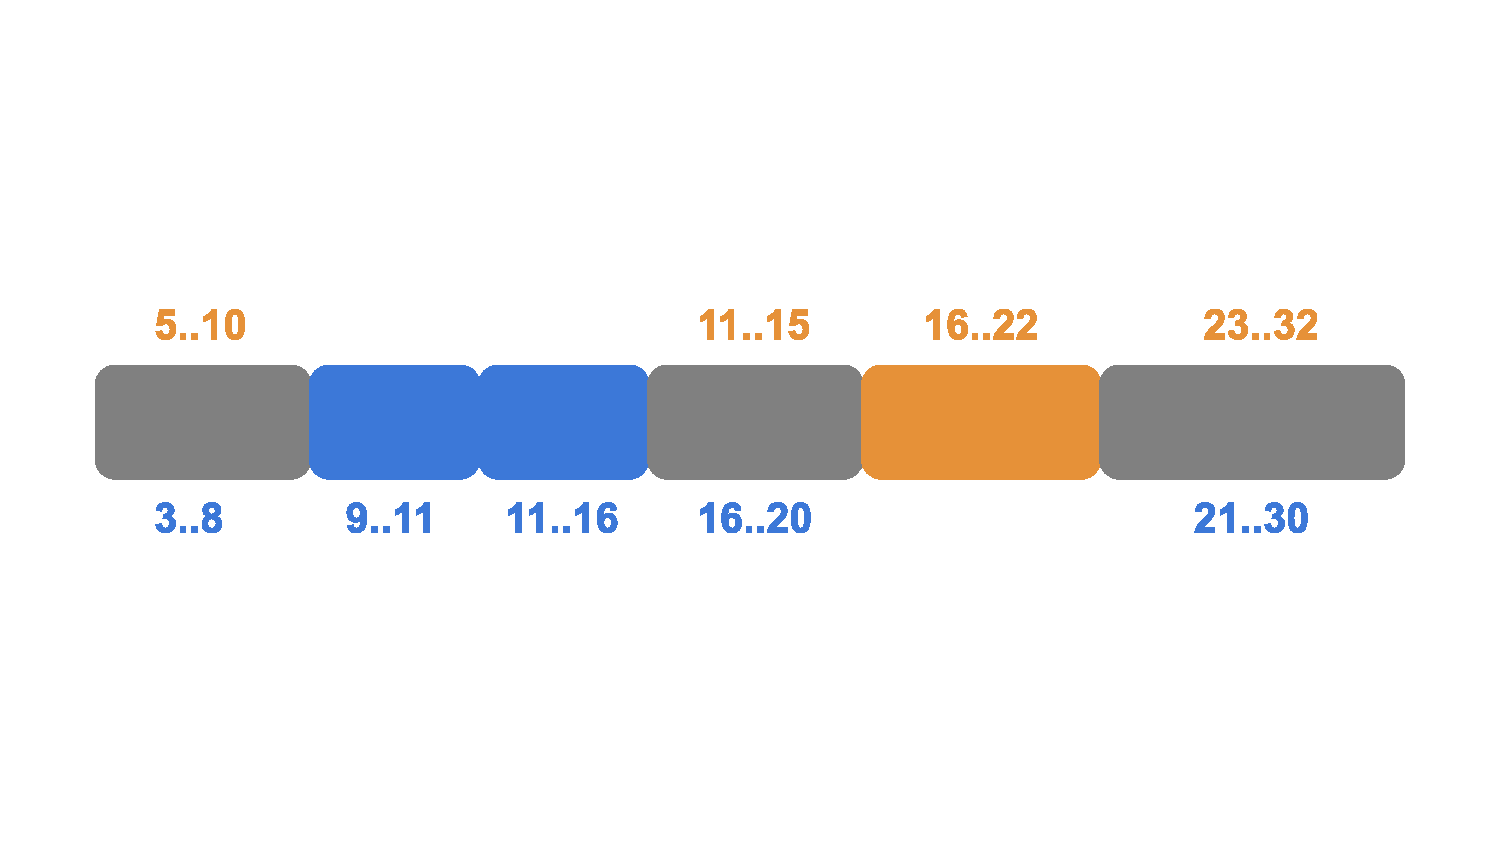
\includegraphics[width=\linewidth]{fig/sketches/1D_sketch_after_update.pdf}
		\label{fig:1d_after_update}
		\end{subfigure}	
		%\smallskip
		\begin{subfigure}[t]{0.32\textwidth}
			\centering
			\caption{}
			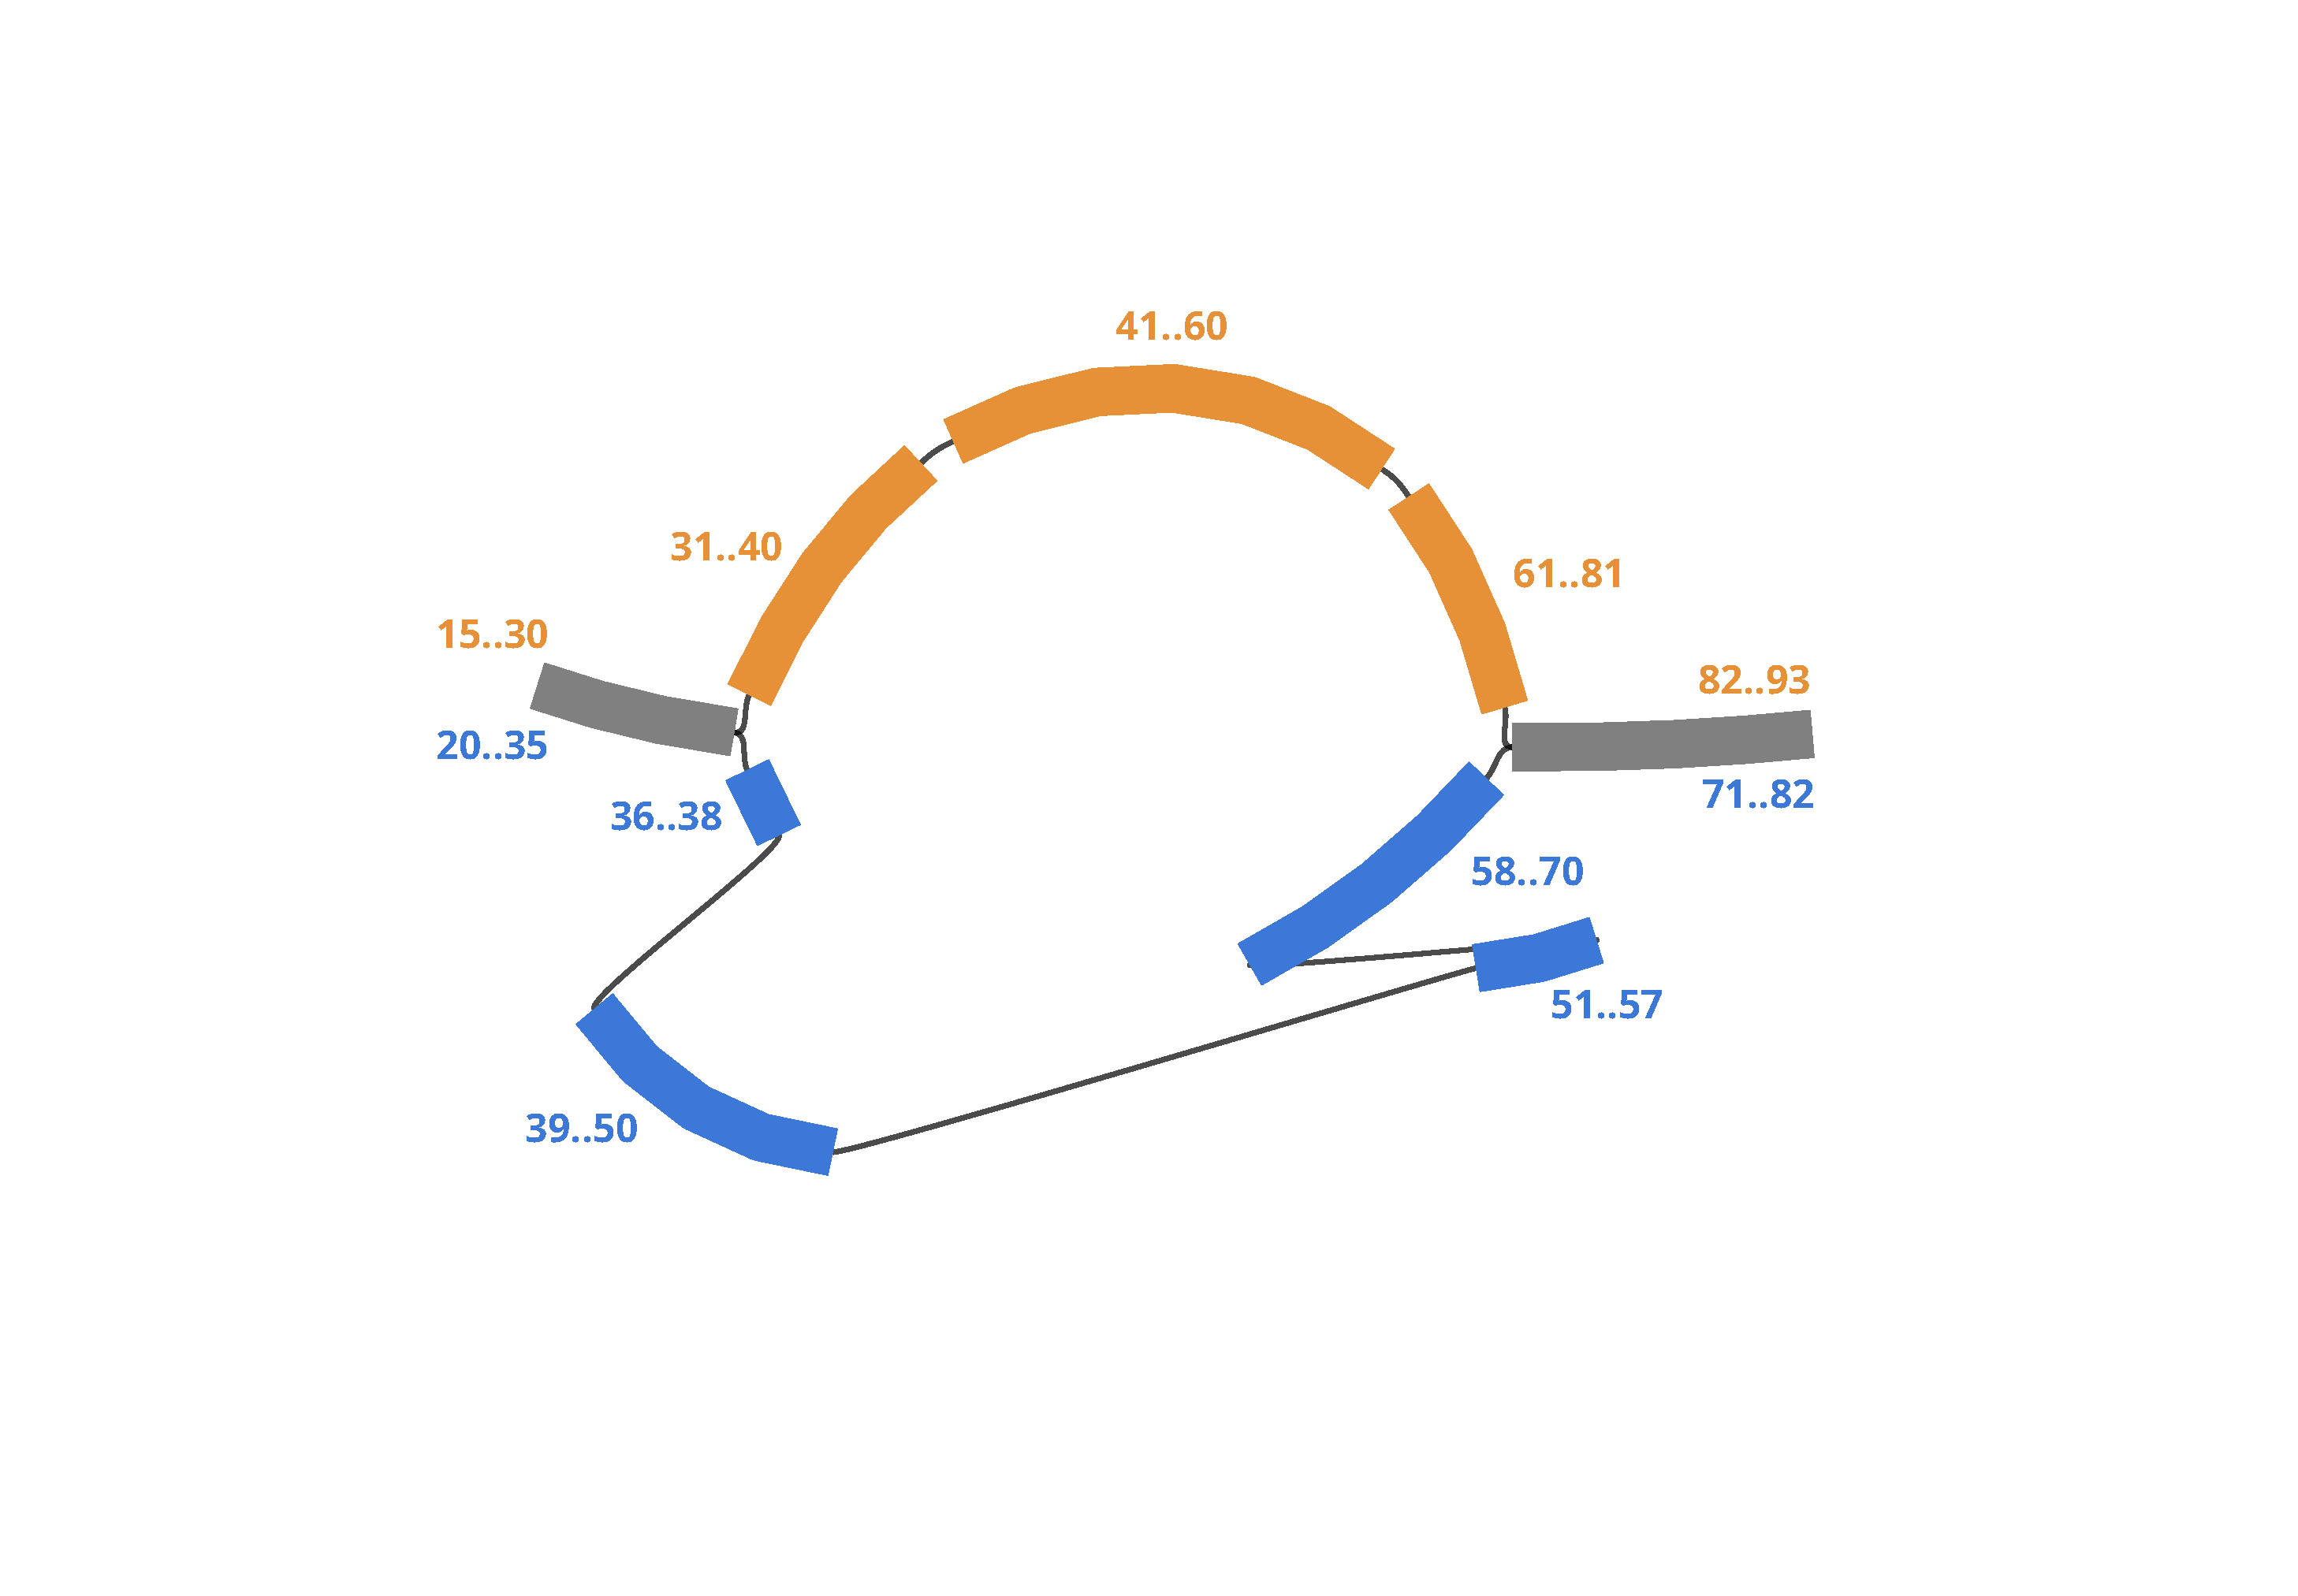
\includegraphics[width=\linewidth]{fig/sketches/2D_sketch_before_update.pdf}
			\label{fig:2d_before_update}
		\end{subfigure}
		\begin{subfigure}[t]{0.32\textwidth}
			\centering
			\caption{}
			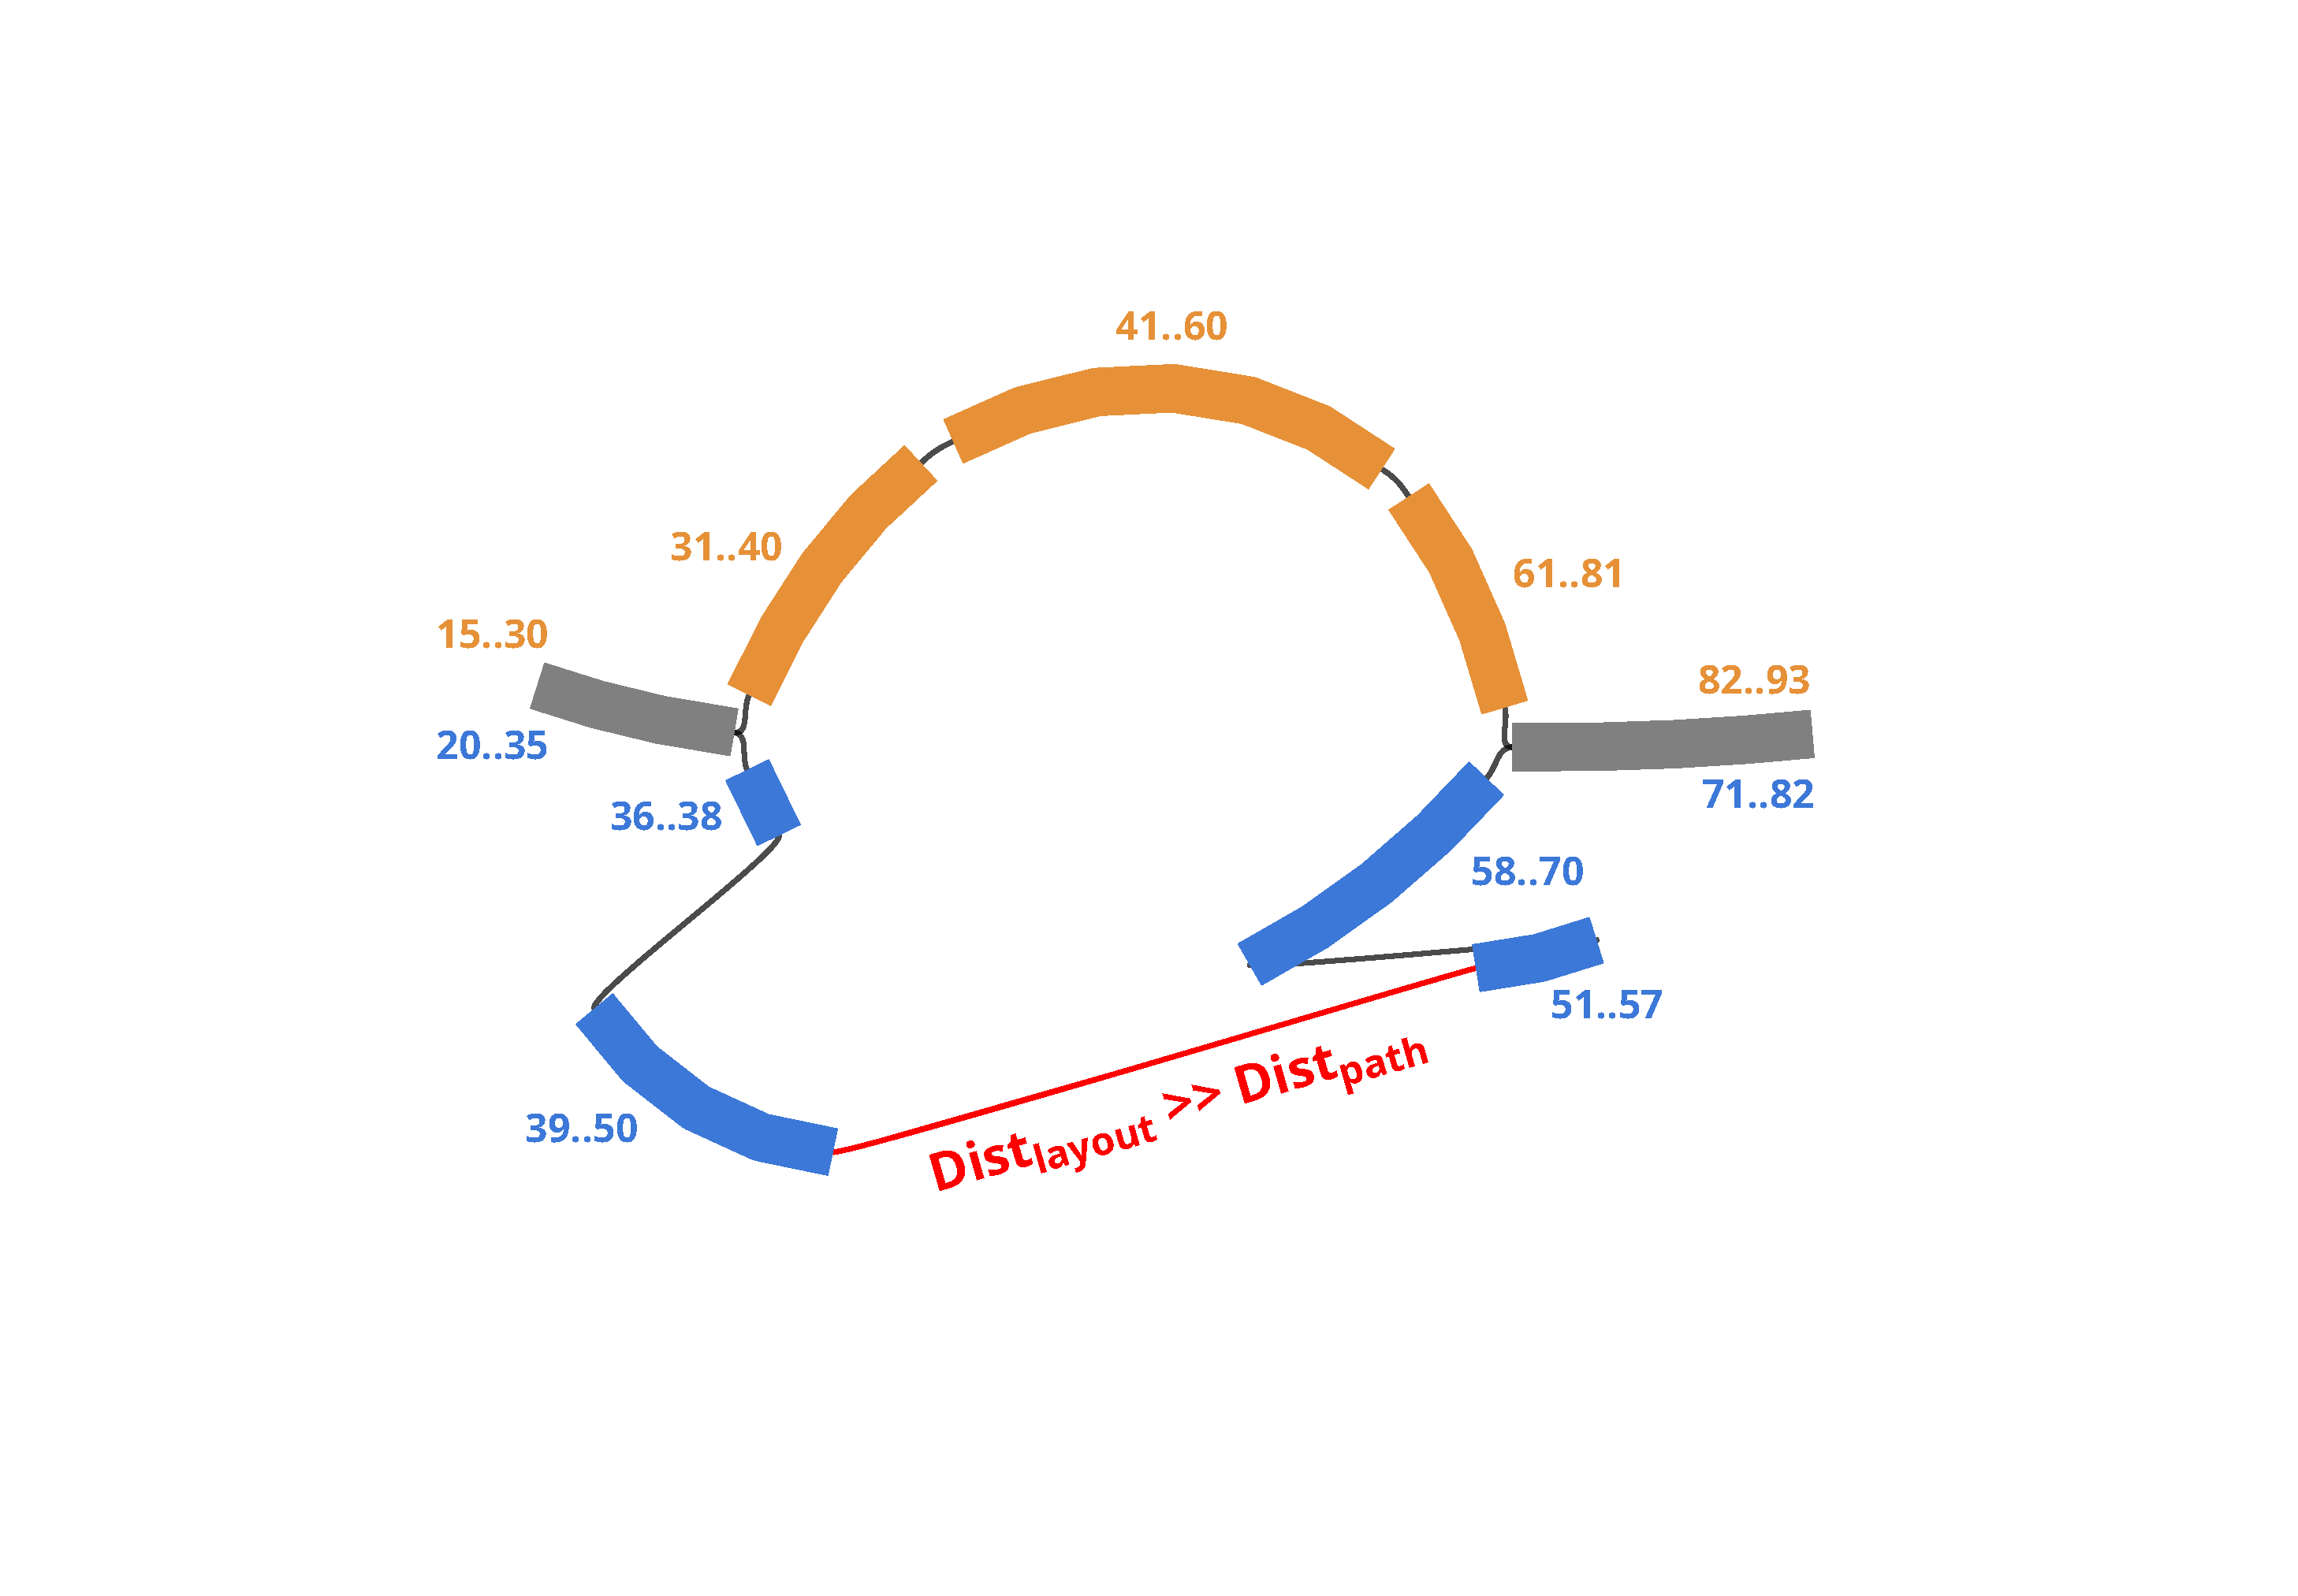
\includegraphics[width=\linewidth]{fig/sketches/2D_sketch_before_update_highlighted.pdf}
			\label{fig:2d_before_update_highlighted}
		\end{subfigure}
		\begin{subfigure}[t]{0.32\textwidth}
		\centering
		\caption{}
		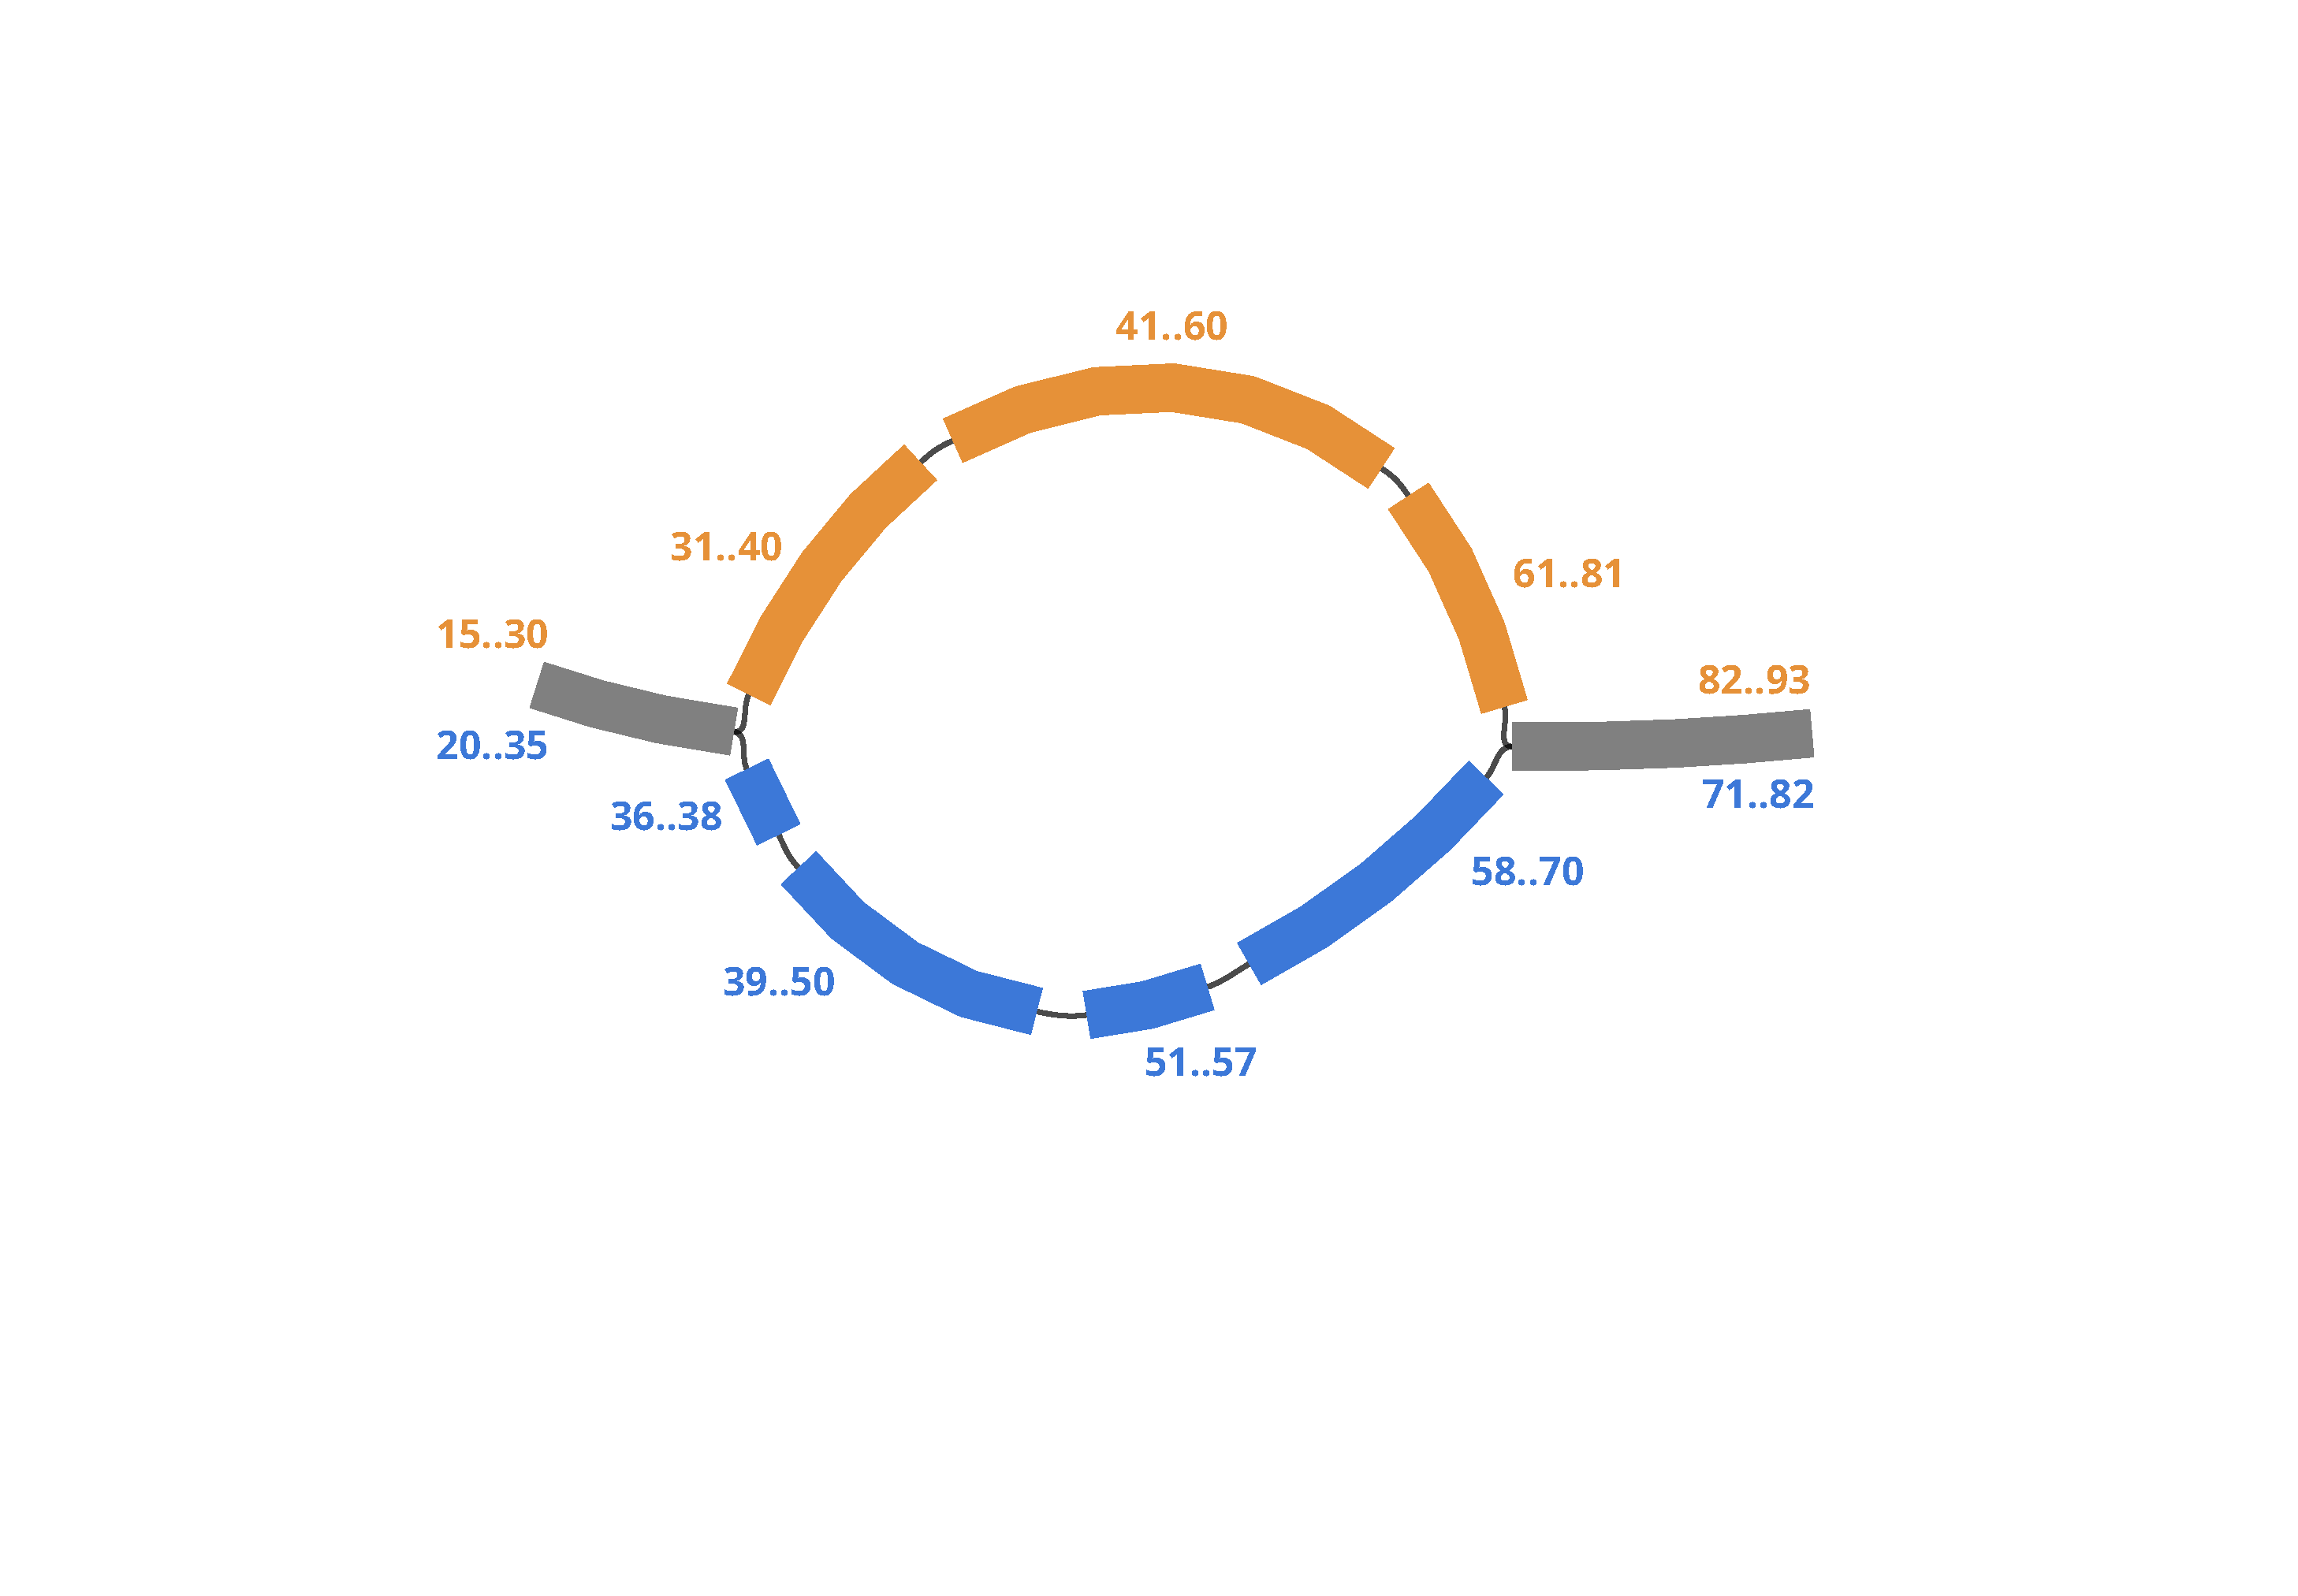
\includegraphics[width=\linewidth]{fig/sketches/2D_sketch_after_update.pdf}
		\label{fig:2d_after_update}
		\end{subfigure}	
	\caption{
		PG-SGD update operation sketches. \textbf{(a)-(c)} 1D layout sketch of an update operation moving a pair of nodes at a time. Edges are not shown. %https://docs.google.com/presentation/d/1Htp2bkCNIXea0QnWuKpi2YzvR4fXppNfLDsihCjcmWM/edit#slide=id.p
		\textbf{(d)-(f)} 2D layout sketch of an update operation moving a pair of nodes at a time. Edges are drawn as black links.
		\textbf{(a)} State of the graph before the 1D update. \textbf{(b)} State of the graph before the update highlighting the discrepancy of the layout distance versus the path nucleotide distance of the blue nodes in 1D.  \textbf{(c)} State of the graph after the 1D update. \textbf{(d)} State of the graph before the 2D update. \textbf{(e)} State of the graph before the update highlighting the discrepancy of the layout distance versus the path nucleotide distance of the blue nodes in 2D. \textbf{(f)} State of the graph after the 2D update.
	}
	\label{fig:sketches}
\end{figure*}